\documentclass{article}

% Required packages
\usepackage{amssymb}
\usepackage{amsmath}
\usepackage{graphicx}
\usepackage{geometry}
\usepackage{tikz}
\usepackage{array}
\usepackage{booktabs}
\usepackage{enumitem}
\usepackage{listings}
\usepackage{xcolor}
\usepackage{subcaption}

% Set page geometry
\geometry{a4paper, margin=1in}

% Configure listings for Python
\lstset{
  language=Python,
  basicstyle=\ttfamily\footnotesize,
  numbers=left,
  numberstyle=\tiny\color{gray},
  frame=single,
  breaklines=true,
  breakatwhitespace=true,
  captionpos=b,
  tabsize=4,
  showspaces=false,
  showstringspaces=false,
  showtabs=false,
  commentstyle=\color{gray}\textit,
  keywordstyle=\color{blue}\bfseries,
  stringstyle=\color{red}
}

% For centering images and tables
\usepackage{float}

\begin{document}

\begin{flushright}
   Randall Rogers\\
   DSC 255: Machine Learning Fundamentals\\
   Homework 3 \\
   Spring 2025 \\
\end{flushright}

\subsection*{Question 1}
\parbox{\textwidth}{Gaussian parameters. Each of the following scenarios describes a joint distribution $(x, y)$. In each case, give the parameters of the (unique) bivariate Gaussian that satisfies these properties.}

\begin{enumerate}[label=(a)]
    \item x has mean 2 and standard deviation 1, y has mean 2 and standard deviation 0.5, and the
correlation between x and y is -0.5.
\end{enumerate}
\begin{enumerate}[label=(b)]
    \item x has mean 1 and standard deviation 1, and y is equal to 2.
\end{enumerate}

\parbox{\textwidth}{\textbf{Solution (a)}}

\noindent\rule{\textwidth}{0.4pt}\\
\parbox{\textwidth}{For a bivariate Gaussian distribution, we need to specify the following parameters:}\\

$$\boldsymbol{\mu} = [\mu_x, \mu_y]^T$$\\
$$\boldsymbol{\Sigma} = \begin{bmatrix} \sigma_x^2 & \rho\sigma_x\sigma_y \\ \rho\sigma_x\sigma_y & \sigma_y^2 \end{bmatrix}$$

\begin{itemize}
    \item Mean vector: $\boldsymbol{\mu}$
    \item Covariance matrix: $\boldsymbol{\Sigma}$
\end{itemize}

\parbox{\textwidth}{Let $\mu_x = 2$, $\mu_y = 2$, $\sigma_x = 1$, $\sigma_y = 0.5$, and $\rho = -0.5$}\\

\parbox{\textwidth}{Solve for mean vector $\boldsymbol{\mu}$:}\\

$$\boldsymbol{\mu} = \begin{bmatrix} \mu_x & \mu_y \end{bmatrix}^T = \begin{bmatrix}
    \mu_x \\
    \mu_y
\end{bmatrix} = \begin{bmatrix}
    2 \\
    2
\end{bmatrix}$$\\

\parbox{\textwidth}{Solve for covariance matrix $\boldsymbol{\Sigma}$:}\\

$$\boldsymbol{\Sigma} = \begin{bmatrix} \sigma_x^2 & \rho\sigma_x\sigma_y \\ \rho\sigma_x\sigma_y & \sigma_y^2 \end{bmatrix} = \begin{bmatrix} 1^2 & (-0.5)(1)(0.5) \\(-0.5)(1)(0.5) & 0.5^2\end{bmatrix} = \begin{bmatrix} 1 & -0.25 \\-0.25 & 0.25\end{bmatrix}$$\\

\parbox{\textwidth}{$\therefore$ the bivariate Gaussian has parameters:}\\

$$\mathcal{N}\left(\begin{bmatrix} 2 \\ 2 \end{bmatrix}, \begin{bmatrix} 
    1 & -0.25 \\
    -0.25 & 0.25
\end{bmatrix}\right)$$

\noindent\rule{\textwidth}{0.4pt}\\

\newpage

\parbox{\textwidth}{\textbf{Solution (b)}}

\noindent\rule{\textwidth}{0.4pt}\\

\parbox{\textwidth}{For a bivariate Gaussian distribution, we need to specify the following parameters:}\\

$$\boldsymbol{\mu} = [\mu_x, \mu_y]^T$$\\
$$\boldsymbol{\Sigma} = \begin{bmatrix} \sigma_x^2 & \rho\sigma_x\sigma_y \\ \rho\sigma_x\sigma_y & \sigma_y^2 \end{bmatrix}$$

\begin{itemize}
    \item Mean vector: $\boldsymbol{\mu}$
    \item Covariance matrix: $\boldsymbol{\Sigma}$
\end{itemize}

\parbox{\textwidth}{Let $\mu_x = 1$, $\mu_y = 2$, $\sigma_x = 1$, $\sigma_y = 0$}\\

\parbox{\textwidth}{Solve for mean vector $\boldsymbol{\mu}$:}\\

$$\boldsymbol{\mu} = \begin{bmatrix} \mu_x & \mu_y \end{bmatrix}^T = \begin{bmatrix}
    \mu_x \\
    \mu_y
\end{bmatrix} = \begin{bmatrix}
    1 \\
    2
\end{bmatrix}$$\\

\parbox{\textwidth}{Solve for covariance matrix $\boldsymbol{\Sigma}$:}\\

$$\boldsymbol{\Sigma} = \begin{bmatrix} \sigma_x^2 & \rho\sigma_x\sigma_y \\ \rho\sigma_x\sigma_y & \sigma_y^2 \end{bmatrix} = \begin{bmatrix} 1^2 & 0 \\ 0 & 0^2\end{bmatrix} = \begin{bmatrix} 1 & 0 \\ 0 & 0\end{bmatrix}$$\\

\parbox{\textwidth}{$\therefore$ the bivariate Gaussian has parameters:}\\

$$\mathcal{N}\left(\begin{bmatrix} 1 \\ 2 \end{bmatrix}, \begin{bmatrix} 
    1 & 0 \\
    0 & 0
\end{bmatrix}\right)$$

\noindent\rule{\textwidth}{0.4pt}\\

\noindent\rule{\textwidth}{0.4pt}\\

\newpage
\subsection*{Question 2}
\parbox{\textwidth}{A generative approach is used for a binary classifcation problem (with classes +, -) and it turns out
that the resulting classifier predicts + at all points x in the input space. Why might this be?}\\

\parbox{\textwidth}{\textbf{Solution}}
\noindent\rule{\textwidth}{0.4pt}\\

\parbox{\textwidth}{\textbf{Step 1:} Recall the Bayesian decision rule for generative classifiers.}

\vspace{0.2cm}

\parbox{\textwidth}{In a generative approach, we model the joint distribution $p(x, y)$ by learning the class-conditional densities $p(x|y)$ and prior probabilities $p(y)$. The classification decision is made using Bayes' rule:}

$$\hat{y} = \arg\max_{y \in \{+,-\}} p(y|x) = \arg\max_{y \in \{+,-\}} \frac{p(x|y)p(y)}{p(x)}$$

\parbox{\textwidth}{Since $p(x)$ is constant for both classes, the decision rule simplifies to:}

$$\hat{y} = \arg\max_{y \in \{+,-\}} p(x|y)p(y)$$

\vspace{0.3cm}

\parbox{\textwidth}{\textbf{Step 2:} Analyze the decision boundary.}

\vspace{0.2cm}

\parbox{\textwidth}{For binary classification, we predict the positive class (+) when:}

$$p(x|+)p(+) > p(x|-)p(-)$$

\parbox{\textwidth}{Equivalently, taking the logarithm (which preserves the inequality since log is monotonically increasing):}

$$\log p(x|+) + \log p(+) > \log p(x|-) + \log p(-)$$

\vspace{0.3cm}

\parbox{\textwidth}{\textbf{Step 3:} Identify possible reasons for always predicting the positive class.}

\vspace{0.2cm}

\parbox{\textwidth}{There are several reasons why the inequality $p(x|+)p(+) > p(x|-)p(-)$ might hold for all $x$:}

\begin{enumerate}
    \item \textbf{Highly imbalanced prior probabilities:} If $p(+) \gg p(-)$, the classifier might always predict the positive class because the prior term dominates the decision, regardless of the likelihood term. This occurs when the training data contains many more positive examples than negative ones.
    
    \item \textbf{Poor estimation of class-conditional densities:} If $p(x|+)$ is consistently overestimated or $p(x|-)$ is consistently underestimated across the input space, the classifier will favor the positive class.
    
    \item \textbf{Model misspecification:} If the assumed parametric form of $p(x|y)$ (e.g., Gaussian) does not match the true distribution of the data, the estimated densities may lead to systematic classification errors.
    
    \item \textbf{Feature insufficiency:} If the selected features do not provide discriminative information to separate the classes, the model might default to the more common class.
    
    \item \textbf{Numerical issues:} In high-dimensional spaces, numerical underflow when computing likelihoods can lead to computational issues that affect the decision boundary.
\end{enumerate}

\vspace{0.3cm}

\parbox{\textwidth}{\textbf{Step 4:} Mathematical illustration with Gaussian class-conditionals.}

\vspace{0.2cm}

\parbox{\textwidth}{For a concrete example, consider a generative classifier with Gaussian class-conditionals:}

$$p(x|+) \sim \mathcal{N}(\mu_+, \Sigma_+)$$
$$p(x|-) \sim \mathcal{N}(\mu_-, \Sigma_-)$$

\parbox{\textwidth}{The decision boundary is determined by:}

$$\log p(x|+) + \log p(+) = \log p(x|-) + \log p(-)$$

\parbox{\textwidth}{Expanding the Gaussian log-likelihoods:}

\begin{align*}
-\frac{1}{2}(x-\mu_+)^T\Sigma_+^{-1}(x-\mu_+) - \frac{1}{2}\log|\Sigma_+| - \frac{d}{2}\log(2\pi) + \log p(+) = \\
-\frac{1}{2}(x-\mu_-)^T\Sigma_-^{-1}(x-\mu_-) - \frac{1}{2}\log|\Sigma_-| - \frac{d}{2}\log(2\pi) + \log p(-)
\end{align*}

\parbox{\textwidth}{If this equation has no solution for any $x$ (i.e., one side is always greater), the classifier will always predict the same class. This can happen if:}

\begin{itemize}
    \item The means $\mu_+$ and $\mu_-$ are very close, but $p(+) \gg p(-)$
    \item The covariance matrices $\Sigma_+$ and $\Sigma_-$ are poorly estimated
    \item The dimensionality $d$ is high relative to the sample size, leading to unreliable parameter estimates
\end{itemize}

\vspace{0.3cm}

\parbox{\textwidth}{\textbf{Conclusion:} A generative classifier that always predicts the positive class indicates an issue with either the data distribution (class imbalance), the model specification, or the parameter estimation process. In practice, this suggests the need to:}

\begin{itemize}
    \item Balance the training data or adjust class priors
    \item Try different parametric forms for the class-conditional densities
    \item Apply regularization to improve parameter estimation
    \item Consider dimensionality reduction if working in high-dimensional spaces
    \item Validate the model's assumptions about the data distribution
\end{itemize}


\noindent\rule{\textwidth}{0.4pt}\\

\noindent\rule{\textwidth}{0.4pt}\\

\newpage

\subsection*{Question 3}
\parbox{\textwidth}{Winery classification. For the winery example from lecture, the densities obtained are reproduced
here:}

\begin{figure}[H]

\includegraphics[width=1\textwidth]{dsc_255_hw3_q3.png} 
\caption{Winery classification densities}
    
\end{figure}

\parbox{\textwidth}{The class probabilities are $\pi_1 = 0.33$; $\pi_2 = 0.39$; $\pi_3 = 0.28$. What labels would be assigned to the
following points?}

\begin{enumerate}[label=(a)]
    \item 12.0
\end{enumerate}
\begin{enumerate}[label=(b)]
    \item 12.5
\end{enumerate}
\begin{enumerate}[label=(c)]
    \item 13.0
\end{enumerate}
\begin{enumerate}[label=(d)]
    \item 13.5
\end{enumerate}
\begin{enumerate}[label=(e)]
    \item 14.0
\end{enumerate}

\parbox{\textwidth}{\textbf{Solution (a)}}
\noindent\rule{\textwidth}{0.4pt}\\

\parbox{\textwidth}{From Bayes Theorem we have:}
$$p(y|x) = \frac{p(x|y)p(y)}{p(x)}$$
$$or$$
$$p(y|x) \propto p(x|y)p(y)$$

\parbox{\textwidth}{The class probabilities are given as: $\pi_1 = 0.33$; $\pi_2 = 0.39$; $\pi_3 = 0.28$}\\

\parbox{\textwidth}{From \textit{Figure 1}, we can see that the density for each class 1 at $x=12.0$ is: $P(x=12.0|Class_1) = 0.4$; for class 2 is $P(x=12.0|Class_2) = 0.05$; and for class 3 is $P(x=12.0|Class_3) = 0.0025$.}\\

\parbox{\textwidth}{Apply Bayes Theorem approimation to solve for $P(Class_i | x=12.0)$}\\

$$P(Class_i|x) \propto P(x|Class_i)P(Class_i)$$

\parbox{\textwidth}{Find $P(Class_i|x=12.0)$ for each class:}\\

$P(Class_1|x=12.0) \propto P(x=12.0|Class_1)P(Class_1) = 0.4 \times 0.33 = 0.132$\\

$P(Class_2|x=12.0) \propto P(x=12.0|Class_2)P(Class_2) = 0.05 \times 0.39 = 0.0195$\\

$P(Class_3|x=12.0) \propto P(x=12.0|Class_3)P(Class_3) = 0.0025 \times 0.28 = 0.0007$\\

\parbox{\textwidth}{$\therefore$ the label $Class_1$ would be assigned at x=12.0}\\

\noindent\rule{\textwidth}{0.4pt}\\

\parbox{\textwidth}{\textbf{Solution (b)}}
\noindent\rule{\textwidth}{0.4pt}\\

\parbox{\textwidth}{From Bayes Theorem we have:}
$$p(y|x) = \frac{p(x|y)p(y)}{p(x)}$$
$$or$$
$$p(y|x) \propto p(x|y)p(y)$$

\parbox{\textwidth}{The class probabilities are given as: $\pi_1 = 0.33$; $\pi_2 = 0.39$; $\pi_3 = 0.28$}\\

\parbox{\textwidth}{From \textit{Figure 1}, we can see that the density for each class 1 at $x=12.5$ is: $P(x=12.5|Class_1) = 0.6$; for class 2 is $P(x=12.5|Class_2) = 0.3$; and for class 3 is $P(x=12.5|Class_3) = 0.05$.}\\

\parbox{\textwidth}{Apply Bayes Theorem approimation to solve for $P(Class_i | x=12.5)$}\\

$$P(Class_i|x) \propto P(x|Class_i)P(Class_i)$$

\parbox{\textwidth}{Find $P(Class_i|x=12.5)$ for each class:}\\

$P(Class_1|x=12.5) \propto P(x=12.5|Class_1)P(Class_1) = 0.6 \times 0.33 = 0.198$\\

$P(Class_2|x=12.5) \propto P(x=12.5|Class_2)P(Class_2) = 0.3 \times 0.39 = 0.117$\\

$P(Class_3|x=12.5) \propto P(x=12.5|Class_3)P(Class_3) = 0.05 \times 0.28 = 0.014$\\

\parbox{\textwidth}{$\therefore$ the label $Class_1$ would be assigned at x=12.5}\\

\noindent\rule{\textwidth}{0.4pt}\\

\parbox{\textwidth}{\textbf{Solution (c)}}
\noindent\rule{\textwidth}{0.4pt}\\

\parbox{\textwidth}{From Bayes Theorem we have:}
$$p(y|x) = \frac{p(x|y)p(y)}{p(x)}$$
$$or$$
$$p(y|x) \propto p(x|y)p(y)$$

\parbox{\textwidth}{The class probabilities are given as: $\pi_1 = 0.33$; $\pi_2 = 0.39$; $\pi_3 = 0.28$}\\

\parbox{\textwidth}{From \textit{Figure 1}, we can see that the density for each class 1 at $x=13.0$ is: $P(x=13.0|Class_1) = 0.3$; for class 2 is $P(x=13.0|Class_2) = 0.6$; and for class 3 is $P(x=13.0|Class_3) = 0.2$.}\\

\parbox{\textwidth}{Apply Bayes Theorem approimation to solve for $P(Class_i | x=13.0)$}\\

\parbox{\textwidth}{Find $P(Class_i|x=13.0)$ for each class:}\\

$$P(Class_i|x) \propto P(x|Class_i)P(Class_i)$$\\

$P(Class_1|x=13.0) \propto P(x=13.0|Class_1)P(Class_1) = 0.3 \times 0.33 = 0.099$\\

$P(Class_2|x=13.0) \propto P(x=13.0|Class_2)P(Class_2) = 0.6 \times 0.39 = 0.234$\\

$P(Class_3|x=13.0) \propto P(x=13.0|Class_3)P(Class_3) = 0.2 \times 0.28 = 0.056$\\

\parbox{\textwidth}{$\therefore$ the label $Class_2$ would be assigned at x=13.0}\\

\noindent\rule{\textwidth}{0.4pt}\\

\parbox{\textwidth}{\textbf{Solution (d)}}
\noindent\rule{\textwidth}{0.4pt}\\

\parbox{\textwidth}{From Bayes Theorem we have:}
$$p(y|x) = \frac{p(x|y)p(y)}{p(x)}$$
$$or$$
$$p(y|x) \propto p(x|y)p(y)$$

\parbox{\textwidth}{The class probabilities are given as: $\pi_1 = 0.33$; $\pi_2 = 0.39$; $\pi_3 = 0.28$}\\

\parbox{\textwidth}{From \textit{Figure 1}, we can see that the density for each class 1 at $x=13.5$ is: $P(x=13.5|Class_1) = 0.1$; for class 2 is $P(x=13.5|Class_2) = 0.7$; and for class 3 is $P(x=13.5|Class_3) = 0.4$.}\\

\parbox{\textwidth}{Apply Bayes Theorem approimation to solve for $P(Class_i | x=13.5)$}\\

\parbox{\textwidth}{Find $P(Class_i|x=13.5)$ for each class:}\\

$$P(Class_i|x) \propto P(x|Class_i)P(Class_i)$$\\

$P(Class_1|x=13.5) \propto P(x=13.5|Class_1)P(Class_1) = 0.1 \times 0.33 = 0.033$\\

$P(Class_2|x=13.5) \propto P(x=13.5|Class_2)P(Class_2) = 0.7 \times 0.39 = 0.273$\\

$P(Class_3|x=13.5) \propto P(x=13.5|Class_3)P(Class_3) = 0.4 \times 0.28 = 0.112$\\

\parbox{\textwidth}{$\therefore$ the label $Class_2$ would be assigned at x=13.5}\\

\noindent\rule{\textwidth}{0.4pt}\\

\parbox{\textwidth}{\textbf{Solution (e)}}
\noindent\rule{\textwidth}{0.4pt}\\

\parbox{\textwidth}{From Bayes Theorem we have:}
$$p(y|x) = \frac{p(x|y)p(y)}{p(x)}$$
$$or$$
$$p(y|x) \propto p(x|y)p(y)$$

\parbox{\textwidth}{The class probabilities are given as: $\pi_1 = 0.33$; $\pi_2 = 0.39$; $\pi_3 = 0.28$}\\

\parbox{\textwidth}{From \textit{Figure 1}, we can see that the density for each class 1 at $x=14.0$ is: $P(x=14.0|Class_1) = 0.05$; for class 2 is $P(x=14.0|Class_2) = 0.2$; and for class 3 is $P(x=14.0|Class_3) = 0.8$.}\\

\parbox{\textwidth}{Apply Bayes Theorem approimation to solve for $P(Class_i | x=14.0)$}\\

\parbox{\textwidth}{Find $P(Class_i|x=14.0)$ for each class:}\\

$$P(Class_i|x) \propto P(x|Class_i)P(Class_i)$$\\

$P(Class_1|x=14.0) \propto P(x=14.0|Class_1)P(Class_1) = 0.05 \times 0.33 = 0.0165$\\

$P(Class_2|x=14.0) \propto P(x=14.0|Class_2)P(Class_2) = 0.2 \times 0.39 = 0.078$\\

$P(Class_3|x=14.0) \propto P(x=14.0|Class_3)P(Class_3) = 0.8 \times 0.28 = 0.224$\\

\parbox{\textwidth}{$\therefore$ the label $Class_3$ would be assigned at x=14.0}\\

\noindent\rule{\textwidth}{0.4pt}\\

\noindent\rule{\textwidth}{0.4pt}\\

\newpage

\subsection*{Question 4}

\parbox{\textwidth}{Gaussian contours. Roughly sketch the shapes of the following Gaussians $N(\mu; \Sigma)$. You only need to show a representative contour line which is qualitatively accurate (has approximately the right orientation, for instance).}\\

\begin{enumerate}[label=(a)]
    \item $\mu = \begin{bmatrix} 0 \\ 0 \end{bmatrix}$; $\Sigma = \begin{bmatrix} 9 & 0 \\ 0 & 1 \end{bmatrix}$\\
\end{enumerate}

\begin{enumerate}[label=(b)]
    \item $\mu = \begin{bmatrix} 0 \\ 0 \end{bmatrix}$; $\Sigma = \begin{bmatrix} 1 & -0.75 \\ -0.75 & 1 \end{bmatrix}$\\
\end{enumerate}

\parbox{\textwidth}{\textbf{Solution (a)}}

\noindent\rule{\textwidth}{0.4pt}\\

\parbox{\textwidth}{Analyze $\mu$:}\\
\begin{itemize}
    \item \parbox{\textwidth}{Since $\mu = \begin{bmatrix} 0 \\ 0 \end{bmatrix}$, the center of the Gaussian is at the origin.}\\
\end{itemize}

\parbox{\textwidth}{Analyze $\Sigma$:}\\

\begin{itemize}
    \item \parbox{\textwidth}{The covariance matrix $\Sigma = \begin{bmatrix} 9 & 0 \\ 0 & 1 \end{bmatrix}$ indicates that the variance in the x-direction is 9 and in the y-direction is 1. This means that the Gaussian will be elongated along the x-axis.}\\
\end{itemize}

\parbox{\textwidth}{Look at the standard deviation to determine the shape, since $\Sigma$ is a diagonal matrix:}\\ 

\begin{itemize}
    \item The standard deviation in the x-direction is $\sigma_x = \sqrt{9} = 3$
    \item The standard deviation in the y-direction is $\sigma_y = \sqrt{1} = 1$
\end{itemize}

\parbox{\textwidth}{Sketch the Gaussian}\\

\begin{center}
    \begin{tikzpicture}
        \draw[->] (-4,0) -- (4,0) node[right] {$x$};
        \draw[->] (0,-2) -- (0,2) node[above] {$y$};
        \draw[thick, blue] (0,0) ellipse (3 and 1);
        \node at (0,0) [circle, fill, inner sep=1pt]{};
        \node at (0.3,0.3) {$\mu$};
        \node at (3.0,0) [circle, fill, inner sep=1pt]{};
        \node at (3.5,0.3) {$\sigma_x = 3$};
        \node at (0,1.0) [circle, fill, inner sep=1pt]{};
        \node at (0.7,1.3) {$\sigma_y = 1$};
    \end{tikzpicture}
\end{center}

\noindent\rule{\textwidth}{0.4pt}\\

\parbox{\textwidth}{\textbf{Solution (b)}}

\noindent\rule{\textwidth}{0.4pt}\\

\parbox{\textwidth}{Analyze $\mu$:}\\
\begin{itemize}
    \item \parbox{\textwidth}{Since $\mu = \begin{bmatrix} 0 \\ 0 \end{bmatrix}$, the center of the Gaussian is at the origin.}\\
\end{itemize}

\parbox{\textwidth}{Analyze $\Sigma$:}\\

\begin{itemize}
    \item The covariance matrix $\Sigma = \begin{bmatrix} 1 & -0.75 \\ -0.75 & 1 \end{bmatrix}$ has non-zero off-diagonal elements.
    \item This indicates a correlation between variables. 
    \item The negative correlation ($-0.75$) means that as one variable increases, the other tends to decrease.\\
    \item Look at the eigenvalues and eigenvectors to determine the shape since we don't have a diagonal matrix in this case.
\end{itemize}

\parbox{\textwidth}{Find eigenvalues and eigenvectors:}\\ 

\begin{itemize}
    \item \parbox{\textwidth}{The eigenvalues of $\Sigma$ are $\lambda_1 = 1 + 0.75 = 1.75$ and $\lambda_2 = 1 - 0.75 = 0.25$.}\\
    \item \parbox{\textwidth}{The corresponding eigenvectors are $v_1 = \begin{bmatrix} 1 \\ -1 \end{bmatrix}$ and $v_2 = \begin{bmatrix} 1 \\ 1 \end{bmatrix}$.}\\
    \item \parbox{\textwidth}{The standard deviations along the principal axes are $\sigma_1 = \sqrt{1.75} \approx 1.32$ and $\sigma_2 = \sqrt{0.25} = 0.5$.}\\
\end{itemize}

\parbox{\textwidth}{Sketch the Gaussian}\\

\begin{center}
    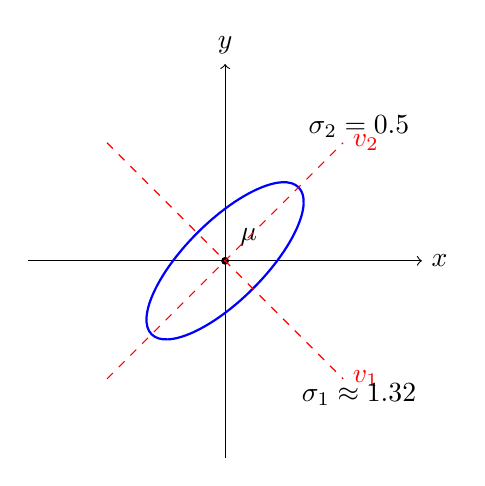
\begin{tikzpicture}
        \draw[->] (-2.5,0) -- (2.5,0) node[right] {$x$};
        \draw[->] (0,-2.5) -- (0,2.5) node[above] {$y$};
        \draw[thick, blue, rotate=45] (0,0) ellipse (1.32 and 0.5);
        \node at (0,0) [circle, fill, inner sep=1pt]{};
        \node at (0.3,0.3) {$\mu$};
        \draw[dashed, red] (-1.5,-1.5) -- (1.5,1.5) node[right] {$v_2$};
        \draw[dashed, red] (-1.5,1.5) -- (1.5,-1.5) node[right] {$v_1$};
        \node at (1.7,-1.7) {$\sigma_1 \approx 1.32$};
        \node at (1.7,1.7) {$\sigma_2 = 0.5$};
    \end{tikzpicture}
\end{center}

\noindent\rule{\textwidth}{0.4pt}\\

\newpage

\subsection*{Question 5}
\parbox{\textwidth}{Find all unit vectors in $\mathbb{R}^2$ that are orthogonal to $\begin{bmatrix} 1 \\ 1 \end{bmatrix}$.}\\
\parbox{\textwidth}{\textbf{Solution}}
\noindent\rule{\textwidth}{0.4pt}\\
\parbox{\textwidth}{A unit vector in $\mathbb{R}^2$ is a vector of the form:}\\
$$\begin{bmatrix} x \\ y \end{bmatrix}$$
\parbox{\textwidth}{To be orthogonal to $\begin{bmatrix} 1 \\ 1 \end{bmatrix}$, the dot product must equal zero:}\\
$$\begin{bmatrix} 1 \\ 1 \end{bmatrix} \cdot \begin{bmatrix} x \\ y \end{bmatrix} = 0$$
\parbox{\textwidth}{This gives the equation:}\\
$$x + y = 0$$
\parbox{\textwidth}{This means that $y = -x$.}\\
\parbox{\textwidth}{Now, we need to find the unit vectors. A unit vector has a magnitude of 1:}\\
$$\sqrt{x^2 + y^2} = 1$$
\parbox{\textwidth}{Substituting $y = -x$ into the equation:}\\
$$\sqrt{x^2 + (-x)^2} = 1$$
$$\sqrt{2x^2} = 1$$
$$\sqrt{2}|x| = 1$$
$$|x| = \frac{1}{\sqrt{2}}$$
\parbox{\textwidth}{This gives two solutions for $x$:}\\
$$x = \frac{1}{\sqrt{2}} \quad \text{or} \quad x = -\frac{1}{\sqrt{2}}$$
\parbox{\textwidth}{Substituting back to find $y$:}\\
$$y = -\frac{1}{\sqrt{2}} \quad \text{or} \quad y = \frac{1}{\sqrt{2}}$$
\parbox{\textwidth}{$\therefore$ the unit vectors orthogonal to $\begin{bmatrix} 1 \\ 1 \end{bmatrix}$ are:}\\
$$\begin{bmatrix} \frac{1}{\sqrt{2}} \\ -\frac{1}{\sqrt{2}} \end{bmatrix} \quad \text{and} \quad \begin{bmatrix} -\frac{1}{\sqrt{2}} \\ \frac{1}{\sqrt{2}} \end{bmatrix}$$

\noindent\rule{\textwidth}{0.4pt}\\

\newpage
\subsection*{Question 6}
\parbox{\textwidth}{How would you describe the set of all points $x$ $\in$ $\mathbb{R}^d$ with $x \cdot x =25$}\\
\parbox{\textwidth}{\textbf{Solution}}
\noindent\rule{\textwidth}{0.4pt}\\
\parbox{\textwidth}{The equation $x \cdot x = 25$ describes a sphere in $\mathbb{R}^d$ with radius 5.}\\
\parbox{\textwidth}{The set of all points $x$ that satisfy this equation is the surface of a sphere centered at the origin with radius 5.}\\
\parbox{\textwidth}{In $d$-dimensional space, the equation can be written as:}\\
$$x_1^2 + x_2^2 + \ldots + x_d^2 = 25$$
\parbox{\textwidth}{This represents a $d$-dimensional sphere (or hypersphere) with radius 5.}\\
\parbox{\textwidth}{The set of all points $x$ that satisfy this equation is the surface of a sphere in $\mathbb{R}^d$.}\\
\parbox{\textwidth}{The surface of the sphere is a $(d-1)$-dimensional manifold embedded in $\mathbb{R}^d$.}\\
\parbox{\textwidth}{In summary, the set of all points $x$ $\in$ $\mathbb{R}^d$ with $x \cdot x = 25$ is a sphere of radius 5 centered at the origin in $d$-dimensional space.}\\
\parbox{\textwidth}{$\therefore$ the set of all points $x$ $\in$ $\mathbb{R}^d$ with $x \cdot x = 25$ is a sphere of radius 5 centered at the origin in $d$-dimensional space.}\\
\noindent\rule{\textwidth}{0.4pt}\\
\noindent\rule{\textwidth}{0.4pt}\\

\newpage
\subsection*{Question 7}
\parbox{\textwidth}{Consider the function $f(x) = 2x_1 -x_2+6x_3$ can be written as $w \cdot x$ for $x$ $\in$ $\mathbb{R}^3$. What is $w$}\\
\parbox{\textwidth}{\textbf{Solution}}
\noindent\rule{\textwidth}{0.4pt}\\

\parbox{\textwidth}{The function $f(x) = 2x_1 - x_2 + 6x_3$ can be expressed in the form of a dot product:}\\

$$f(x) = w \cdot x$$\\

\parbox{\textwidth}{Where $w$ is a vector in $\mathbb{R}^3$ and $x$ is a vector in $\mathbb{R}^3$.}\\

\parbox{\textwidth}{We can then express $f(x)$ as the dot product of two matrices:}\\

$$f(x) = \begin{bmatrix} w_1 \\ w_2 \\ w_3 \end{bmatrix} \cdot \begin{bmatrix} x_1 \\ x_2 \\ x_3 \end{bmatrix} = w_1\cdot x_1 +w_2\cdot x_2 +w_3\cdot x_3$$

\parbox{\textwidth}{It follows that: $w_1 = 2 \hspace{0.2cm} w_2=-1 \hspace{0.2cm} w_3 = 6$}\\

\parbox{\textwidth}{$\therefore$ the vector $w$ is:}\\

$$w = \begin{bmatrix} 2 \\ -1 \\ 6 \end{bmatrix}$$

\noindent\rule{\textwidth}{0.4pt}\\
\noindent\rule{\textwidth}{0.4pt}\\

\newpage
\subsection*{Question 8}
\parbox{\textwidth}{For a certain pair of matrices $A$, $B$ the product $AB$ has dimension $10 \times 20$. If $A$ has $30$ columns, what are the dimensions of $A$ and $B$?}\\

\parbox{\textwidth}{\textbf{Solution}}
\noindent\rule{\textwidth}{0.4pt}\\

\parbox{\textwidth}{Let the dimensions of $A$ be $m \times n$ and the dimensions of $B$ be $n \times p$.}\\

\parbox{\textwidth}{The product $AB$ will have dimensions $m \times p$.}\\

\parbox{\textwidth}{Given that $AB$ has dimensions $10 \times 20$, and $A = m \times 30$:}\\
$$m = 10 \quad \text{and} \quad p = 20$$
\parbox{\textwidth}{Also, we know that $A$ has $30$ columns, which means:}\\
$$n = 30$$
\parbox{\textwidth}{$\therefore$ the dimensions of $A$ and $B$ are:}\\
$$A: 10 \times 30$$
$$B: 30 \times 20$$

\noindent\rule{\textwidth}{0.4pt}\\
\noindent\rule{\textwidth}{0.4pt}\\

\newpage

\subsection*{Question 9}
\parbox{\textwidth}{We have $n$ data points $x^{(1)}$,...,$x^{(n)}$ $\in \mathbb{R}^d$ and we store them in a matrix $X$, one point per row.}\\
$$X = \begin{bmatrix}
x^{(1)} \\
x^{(2)} \\
\vdots \\
x^{(n)}
\end{bmatrix}$$

\begin{enumerate}[label=(a)]
    \item What is the dimension of $X$, in terms of n and d?
\end{enumerate}

\begin{enumerate}[label=(b)]
    \item What is the dimension of ${XX}^T$?
\end{enumerate}

\begin{enumerate}[label=(c)]
    \item What is the $(i,j)$ entry of  ${X}^TX$, simply?
\end{enumerate}

\parbox{\textwidth}{\textbf{Solution (a)}}

\noindent\rule{\textwidth}{0.4pt}\\

\parbox{\textwidth}{The matrix $X$ has $n$ rows and $d$ columns, so the dimension of $X$ is:}\\

$$X \in \mathbb{R}^{n \times d}$$

\parbox{\textwidth}{This means that $X$ has $n$ data points, each with $d$ features.}\\

\parbox{\textwidth}{$\therefore$ the dimension of $X$ is $n \times d$.}\\

\noindent\rule{\textwidth}{0.4pt}\\

\parbox{\textwidth}{\textbf{Solution (b)}}

\noindent\rule{\textwidth}{0.4pt}\\

\parbox{\textwidth}{The matrix ${XX}^T$ is the product of an $n \times d$ matrix and a $d \times n$ matrix.}\\

\parbox{\textwidth}{The resulting matrix will have dimensions $n \times n$.}\\

\parbox{\textwidth}{$\therefore$ the dimension of ${XX}^T$ is $n \times n$.}\\

\noindent\rule{\textwidth}{0.4pt}\\

\parbox{\textwidth}{\textbf{Solution (c)}}

\noindent\rule{\textwidth}{0.4pt}\\

\parbox{\textwidth}{The $(i,j)$ entry of ${X}^TX$ is the dot product of the $i$-th row of $X$ and the $j$-th column of $X^T$ }\\

\parbox{\textwidth}{This is simply the sum of the products of the corresponding elements:}\\

$$(X^TX)_{ij} = \sum_{k=1}^{d} x^{(i)}_k x^{(j)}_k$$

\parbox{\textwidth}{This is the inner product of the $i$-th and $j$-th data points.}\\

\parbox{\textwidth}{$\therefore$ the $(i,j)$ entry of ${X}^TX$ is the inner product of the $i$-th and $j$-th data points or $(x^{(n)},x^{(n)})$.}\\

\noindent\rule{\textwidth}{0.4pt}\\
\noindent\rule{\textwidth}{0.4pt}\\

\newpage

\subsection*{Question 10}

\parbox{\textwidth}{For $x = \begin{bmatrix} 1\\ 3 \\ 5 \end{bmatrix}$, compute $x^Tx$ and $xx^T$.}\\

\parbox{\textwidth}{\textbf{Solution}}

\noindent\rule{\textwidth}{0.4pt}\\

\parbox{\textwidth}{The vector $x$ is:}\\

$$x = \begin{bmatrix} 1 \\ 3 \\ 5 \end{bmatrix}$$

\parbox{\textwidth}{To compute $x^Tx$:}\\

$$x^Tx = \begin{bmatrix} 1 & 3 & 5 \end{bmatrix} \begin{bmatrix} 1 \\ 3 \\ 5 \end{bmatrix}$$

\parbox{\textwidth}{This is the dot product of $x$ with itself:}\\

$$x^Tx = 1^2 + 3^2 + 5^2 = 1 + 9 + 25 = 35$$

\parbox{\textwidth}{To compute $xx^T$:}\\

$$xx^T = \begin{bmatrix} 1 \\ 3 \\ 5 \end{bmatrix} \begin{bmatrix} 1 & 3 & 5 \end{bmatrix}$$

\parbox{\textwidth}{This is the outer product of $x$ with itself:}\\

$$xx^T = \begin{bmatrix} 1 \\ 3 \\ 5 \end{bmatrix} \begin{bmatrix} 1 & 3 & 5 \end{bmatrix} = \begin{bmatrix} 1 & 3 & 5 \\ 3 & 9 & 15 \\ 5 & 15 & 25 \end{bmatrix}$$

\parbox{\textwidth}{$\therefore$ the results are:}\\

$$x^Tx = 35$$

$$xx^T = \begin{bmatrix} 1 & 3 & 5 \\ 3 & 9 & 15 \\ 5 & 15 & 25 \end{bmatrix}$$

\noindent\rule{\textwidth}{0.4pt}\\
\noindent\rule{\textwidth}{0.4pt}\\

\newpage

\subsection*{Question 11}

\parbox{\textwidth}{The quadratic function $f : \mathbb{R}^3 \rightarrow \mathbb{R}$ given by:}\\

$$f(x) = 3x^2_1 +2x_1x_2 -4x_1x_3 +6x^2_3$$\\

\parbox{\textwidth}{can be written in the form $x^TMx$ for some symmetic matrix $M$. What is $M$?}\\

\parbox{\textwidth}{\textbf{Solution}}

\noindent\rule{\textwidth}{0.4pt}\\

\parbox{\textwidth}{The quadratic function can be expressed in the form:}\\

$$f(x) = x^TMx$$

\parbox{\textwidth}{Where $x = \begin{bmatrix} x_1 \\ x_2 \\ x_3 \end{bmatrix}$ and $M$ is a symmetric matrix.}\\

\parbox{\textwidth}{To find the matrix $M$, we can rewrite the quadratic function in matrix form:}\\

$$f(x) = \begin{bmatrix} x_1 & x_2 & x_3 \end{bmatrix} \begin{bmatrix} 3 & 1 & -2 \\ 1 & 0 & 0 \\ -2 & 0 & 6 \end{bmatrix} \begin{bmatrix} x_1 \\ x_2 \\ x_3 \end{bmatrix}$$

\parbox{\textwidth}{This gives us the matrix $M$:}\\

$$M = \begin{bmatrix} 3 & 1 & -2 \\ 1 & 0 & 0 \\ -2 & 0 & 6 \end{bmatrix}$$

\parbox{\textwidth}{To ensure that $M$ is symmetric, we can check that $M = M^T$:}\\

$$M^T = \begin{bmatrix} 3 & 1 & -2 \\ 1 & 0 & 0 \\ -2 & 0 & 6 \end{bmatrix}$$

\parbox{\textwidth}{This confirms that $M$ is symmetric.}\\

\parbox{\textwidth}{$\therefore$ the matrix $M$ is:}\\

$$M = \begin{bmatrix} 3 & 1 & -2 \\ 1 & 0 & 0 \\ -2 & 0 & 6 \end{bmatrix}$$

\noindent\rule{\textwidth}{0.4pt}\\

\noindent\rule{\textwidth}{0.4pt}\\

\newpage

\subsection*{Question 12}

\parbox{\textwidth}{Let $A= diag(1,2,3,4,5,6,7,8)$:}\\

$$A = \begin{bmatrix}
    1 & 0 & 0 & 0 & 0 & 0 & 0 & 0 \\
    0 & 2 & 0 & 0 & 0 & 0 & 0 & 0 \\
    0 & 0 & 3 & 0 & 0 & 0 & 0 & 0 \\
    0 & 0 & 0 & 4 & 0 & 0 & 0 & 0 \\
    0 & 0 & 0 & 0 & 5 & 0 & 0 & 0 \\
    0 & 0 & 0 & 0 & 0 & 6 & 0 & 0 \\
    0 & 0 & 0 & 0 & 0 & 0 & 7 & 0 \\
    0 & 0 & 0 & 0 & 0 & 0 & 0 & 8
\end{bmatrix}$$

\begin{enumerate}[label=(a)]
    \item What is $|A|$?
\end{enumerate}

\begin{enumerate}[label=(b)]
    \item What is $A^{-1}$?
\end{enumerate}

\parbox{\textwidth}{\textbf{Solution (a)}}
\noindent\rule{\textwidth}{0.4pt}\\
\parbox{\textwidth}{The determinant of a diagonal matrix is the product of its diagonal elements:}\\

$$|A| = 1 \cdot 2 \cdot 3 \cdot 4 \cdot 5 \cdot 6 \cdot 7 \cdot 8 = 8! = 40320$$

\parbox{\textwidth}{$\therefore$ the determinant of $A= 40320$}\\

\noindent\rule{\textwidth}{0.4pt}\\
\parbox{\textwidth}{\textbf{Solution (b)}}
\noindent\rule{\textwidth}{0.4pt}\\
\parbox{\textwidth}{The inverse of a diagonal matrix is obtained by taking the reciprocal of each diagonal element:}\\
$$A^{-1} = diag\left(\frac{1}{1}, \frac{1}{2}, \frac{1}{3}, \frac{1}{4}, \frac{1}{5}, \frac{1}{6}, \frac{1}{7}, \frac{1}{8}\right)$$

\parbox{\textwidth}{$\therefore$ the inverse of $A$ is:}\\
$$A^{-1} = \begin{bmatrix}
    1 & 0 & 0 & 0 & 0 & 0 & 0 & 0 \\
    0 & \frac{1}{2} & 0 & 0 & 0 & 0 & 0 & 0 \\
    0 & 0 & \frac{1}{3} & 0 & 0 & 0 & 0 & 0 \\
    0 & 0 & 0 & \frac{1}{4} & 0 & 0 & 0 & 0 \\
    0 & 0 & 0 & 0 & \frac{1}{5} & 0 & 0 & 0 \\
    0 & 0 & 0 & 0 & 0 & \frac{1}{6} & 0 & 0 \\
    0 & 0 & 0 & 0 & 0 & 0 & \frac{1}{7} & 0 \\
    0 & 0 & 0 & 0 & 0 & 0 & 0 & \frac{1}{8}
\end{bmatrix}$$
\noindent\rule{\textwidth}{0.4pt}\\
\noindent\rule{\textwidth}{0.4pt}\\

\newpage

\subsection*{Programming Exercises}

\subsection*{Question 13}
\parbox{\textwidth}{Classifying MNIST digits using generative modeling. In class, we have already encountered the MNIST data set of handwritten digits.
In this problem, you will build a classifier for this data, by modeling each class as a multivariate (784-dimensional) Gaussian.}

\begin{itemize}
    \item Download the Jupyter notebook \texttt{generative-mnist.ipynb} from the course website.
    Look over the notebook to see what it is doing, and then run it, one cell at a time.
    Make sure you understand the form in which the training and test data are stored.
    Towards the end of the notebook, there is also a helper function that displays digits.

    \item Split the training set into two pieces a training set of size 50000 (say), and a separate validation set of size 10000.

    \item Now fit a Gaussian generative model to the training data of 50000 points.
    Determine the class probabilities: what fraction $\pi_{0}$ of the training points are digit 0, for instance?
    Call these values $\pi_{0},...,\pi_{9}$.
    Fit a Gaussian to each digit, by finding the mean and the covariance of the corresponding data points.
    Let the Gaussian for the jth digit be $P_{j}=N(\mu_{j},\Sigma_{j})$.
    Note that $\mu_{j}$ will be a 784-dimensional vector, and $\Sigma_{j}$ will be a $784\times784$ matrix.
    Using these two pieces of information, you can classify new images using Bayes' rule: simply pick the digit j for which $\pi_{j}P_{j}(x)$ is largest.

    \item One last step is needed: it is important to smooth the covariance matrices, and the usual way to do this is to add in $cI$, where c is some constant and I is the identity matrix.
    Use the validation set to help you choose the right value of c: that is, choose the value of c for which the resulting classifier makes the fewest mistakes on the validation set.

    \item There are some important details of numerical precision that deserve attention.
    In 784-dimensional space, all probabilities $P_{j}(x)$ will likely be miniscule, and this can produce all sorts of trouble due to underflow errors.
    It is better to work with log-probabilities: 1000 is easier to deal with than $e^{-1000}$.
    This means that you should classify a point by picking the j that maximizes $log~\pi_{j}+log~P_{j}(x).$
    Fortunately, the Python multivariate normal package will directly compute $log~P_{j}(x)$ for you.

    \item To turn in:

    \begin{enumerate}
        \item[(a)] Pseudocode for your training procedure, making it clear how the validation set was created and used.
        \item[(b)] Did you use a single value of c for all ten classes, or separate values for each class?
        What value(s) of c did you get?
        \item[(c)] What was the error rate on the MNIST test set?
        \item[(d)] Out of the misclassified test digits, pick five at random and display them.
    \end{enumerate}
\end{itemize}

\newpage

\parbox{\textwidth}{\textbf{13 (a)}}

\noindent\rule{\textwidth}{0.4pt}\\

\parbox{\textwidth}{Pseudocode for training procedure:}\\
\begin{enumerate}
\item Input
\begin{itemize}
    \item x: training data
    \item y: training labels
    \item c: smoothing constant for covariance matrices
\end{itemize}
\item Initialize
\begin{itemize}
    \item x\_train: 80\% of x
    \item x\_val: 20\% of x
    \item y\_train: 80\% of y
    \item y\_val: 20\% of y
    \item $\pi_k$: class $k$ frequencies
    \item $\mu_k$: class $k$ mean vector
    \item $\Sigma_k$: class $k$ covariance matrices
    \item qda: Gaussian generative model
\end{itemize}
\item Iterate
\begin{itemize}
    \item For each class $k$ in {0, 1, ..., 9}:
    \begin{itemize}
        \item Compute $\pi_k$ as the fraction of training points in class $k$
        \item Compute $\mu_k$ as the mean of training points in class $k$
        \item Compute $\Sigma_k$ as the covariance of training points in class $k$
        \item Smooth $\Sigma_k$ by adding $cI$ to it
        \item Store each $\pi_k$, $\mu_k$, and $\Sigma_k$
    \end{itemize}
\end{itemize}
\item Evaluate
\begin{itemize}
    \item For each point in the validation set(x\_val) and each c value tested:
    \begin{itemize}
        \item Compute average accuracy of the model over all classes
        \item Store the accuracy for each c value
        \item Choose the c value that gives the best accuracy
        \item Store the best c value
    \end{itemize}
    \item Compute the final model using the best c value
    \item Store each $\pi_k$, $\mu_k$, and $\Sigma_k$ for the final model
\end{itemize}
\end{enumerate}

\newpage
\parbox{\textwidth}{\textbf{13 (b)}}
\noindent\rule{\textwidth}{0.4pt}\\
\begin{itemize}
    \item \parbox{\textwidth}{A single value of $c=0.95$ for all ten classes.}\\
    \item \parbox{\textwidth}{The value of $c$ was chosen based on the validation set accuracy.}\\
    \item \parbox{\textwidth}{The accuracy for $c=0.95$ was $0.8742$ or 87.42\%.}\\
\end{itemize}

\begin{figure}[H]
\includegraphics[width=1\textwidth]{hw3_13_b.png} 
\caption{Results from c value testing}
\end{figure}
\noindent\rule{\textwidth}{0.4pt}\\
\newpage
\parbox{\textwidth}{\textbf{13 (c)}}
\noindent\rule{\textwidth}{0.4pt}\\
\begin{itemize}
    \item \parbox{\textwidth}{The model with $c=0.95$ predicted 1178 out of 10,000 incorrectly.}\\
    \item \parbox{\textwidth}{Therefore, the error rate on the MNIST test set was 0.1178 or 11.78\%.}\\
    \item \parbox{\textwidth}{Note: The accuracy of the model on the MNIST test set (88.22\%) was very close to accuracy on the training set(87.42)\%.}\\
\end{itemize}

\newpage
\parbox{\textwidth}{\textbf{13 (d)}}

\noindent\rule{\textwidth}{0.4pt}\\
\begin{figure}[H]
    \centering
    \begin{subfigure}[b]{0.3\textwidth}
        \centering
        \includegraphics[width=\textwidth]{digit1.png}
        \caption{5 classified as 3}
        \label{fig:digit1}
    \end{subfigure}
    \hfill
    \begin{subfigure}[b]{0.3\textwidth}
        \centering
        \includegraphics[width=\textwidth]{digit2.png}
        \caption{3 classified as 2}
        \label{fig:digit2}
    \end{subfigure}
    \hfill
    \begin{subfigure}[b]{0.3\textwidth}
        \centering
        \includegraphics[width=\textwidth]{digit3.png}
        \caption{5 classified as 8}
        \label{fig:digit3}
    \end{subfigure}
    
    \vspace{1cm}
    
    \begin{subfigure}[b]{0.3\textwidth}
        \centering
        \includegraphics[width=\textwidth]{digit4.png}
        \caption{1 classified as 8}
        \label{fig:digit4}
    \end{subfigure}
    \hfill
    \begin{subfigure}[b]{0.3\textwidth}
        \centering
        \includegraphics[width=\textwidth]{digit5.png}
        \caption{5 classified as 8}
        \label{fig:digit5}
    \end{subfigure}

    \caption{Examples of misclassified digits from the test set}
    \label{fig:misclassified}
\end{figure}

\end{document}